\documentclass[]{article}

\usepackage[margin=1.0in]{geometry}
\usepackage[]{graphicx}
\usepackage{cite}

\newcommand\tab[1][1cm]{\hspace*{#1}}

\begin{document}


\includegraphics[scale=0.1]{res/epoka.png}
\\
\begin{center}
	\begin{large}
		\textbf{
		CEN 350 - Theory of Computation\\
		Louis Alban Ziko\\
		Assignment Report - Levenstein Algorithm\\
		}
	\end{large}
	\begin{small}
		\textbf{Checking the similarities between files\\}
	\end{small}
\end{center}
\section{Abstract}
\tab This assigment involved writing a program which would find the
similarities between 10 DNA files. The files were 100 characters long 
and were randomly generated. The program would check each of the files
against each other to form a table of how similar they are to each other.

\section{Introduction}
\tab \textbf{Levenstein Algorithm} is used for finding the difference between
two strings. It finds a number which is the minimum number of changes required
to change the first string into the second. The time complexity of the algorithm
depends on the length of the two strings being compared. So if the lengths are 
$m$ and $n$ the time complexity is $\mathcal{O}(n*m)$ since we have to go through
all the pairs of characters from the two strings.

\section{Dataset}
\tab As instructed I generated 10 random DNA sequences from 'https://faculty.ucr.edu/~mmaduro/random.htm'
which I then saved into 10 different files which are stored with the code under
the 'files' folder.

\section{Experiments and Results}

\subsection{Task 1}
\tab The first task involved creating the 10 files.

\subsection{Task 2}
\tab The second task involved writing a program which utilized the Levenstein
algorithm to find the similarities between the created files.\\
\tab To do this I used python because it easy to use and doesn't require a
compiler. Also I found an implementation of the Levenstein algorithm at the
following website \cite{LevensteinCode}. By using the function written I was able to pass each 
of the contents of the files in pairs and form a table which showed the results.

\subsection{Task 3}
\tab The third task involved showing the resulting table:\\ \\
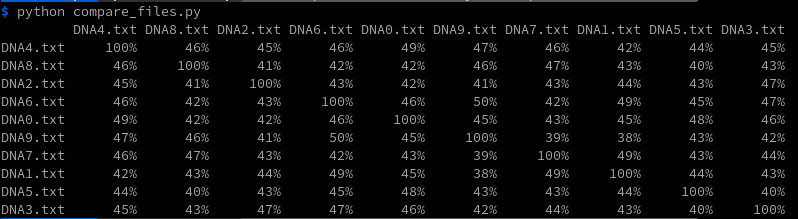
\includegraphics[scale=0.7]{res/similarities.png}

\subsection{Task 5}
\tab The fifth task involved finding the 3 most similar files to the first file.
Let's take 'DNA4.txt' as the first file since it appears first in the table.
Then the most similar files to it, according to the table, are:
\begin{enumerate}
	\item DNA0.txt with 49\%
	\item DNA9.txt with 47\%
	\item DNA8.txt, DNA6.txt and DNA7.txt with 46\%
\end{enumerate}

\bibliography{references}{}
\bibliographystyle{plain}

\end{document}